\begin{slide}
\begin{center}\Title{Our requirements}\end{center}

\begin{itemize}

\IncPart{1}{\item[]
``Expanding'' requires two features.
The construct $\IRef{h}T$ representing
the delayed lift of the term $T$ by $\Uniform{h}$
and $\beta$-reduction at a distance.
}

\IncPart{2}{\item[]
This $\beta$-reduction appears first in Nederpelt's works
and for instance allows the step:
$\Comp{\Abst{x_1}\Abst{x_2}T}\Appl{V_1}\Appl{V_2} \BDStep
\Comp{\Abst{x_1}T\Subs{V_2}{x_2}}\Appl{V_1}
$.
}

\IncPart{3}{\item[]
``Focused'' requires to single out
the instance of the variable we want to replace.
To this aim we use a \stress{path in the redex a.s.t.}
}

\IncPart{4}{\item[]
The a.s.t.'s we are proposing
have no labels on nodes, just on edges.
}

\IncPart{4}{\item[]
\begin{center}
\begin{tabular}{cccc}
$T\Appl{V}$
&
$\Abst{}T$
&
$\IRef{h}T$
&
$n$
\\
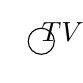
\begin{tikzpicture}[baseline=0pc]
\tikzset{level distance=5pc}
\Tree
[.\node[draw,circle]{};
  \edge node[left]{$\LabA$}; $T$
  \edge node[right]{$\LabS$}; $V$
]
\end{tikzpicture}
&
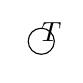
\begin{tikzpicture}[baseline=0pc]
\tikzset{level distance=5pc}
\Tree
[.\node[draw,circle]{};
  \edge node[right]{$\LabL$}; $T$
]
\end{tikzpicture}
&
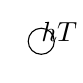
\begin{tikzpicture}[baseline=0pc]
\tikzset{level distance=5pc}
\Tree
[.\node[draw,circle]{};
  \edge node[right]{$\LabD{h}$}; $T$
]
\end{tikzpicture}
&
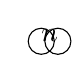
\begin{tikzpicture}[baseline=0pc]
\tikzset{level distance=4.25pc}
\Tree
[.\node[draw,circle]{};
  \edge node[right]{$\LabD{n}$};
  \node[draw,circle]{};
]
\end{tikzpicture}
\\
\end{tabular}
\end{center}
}

\IncPart{5}{\item[]
We denote a path by the labels of its edges
listed from the root (left end) to the leaf (right end).
E.g., the path to the leaf $\mstress{1}$ is: $\IS\LabA\LabL\LabS\LabD{1}$.
}

\IncPart{6}{\item[]
Once paths are introduced, representing a term
as the \stress{set of all paths in its a.s.t.}
allows to operate easily on a single path.
}

\end{itemize}

\end{slide}
